\section{自主实验结果与分析}\label{sec:m2-results}
\subsection{验证集结果与正向系数选择}
四组共20次训练及所有Probe均完整完成，训练和验证损失没有NaN或Inf。表\ref{tab:m2-validation}及图\ref{fig:m2-validation}显示，各正向系数的验证均值均低于均匀控制组，且在本次三个候选值上随系数增大而下降。

令$v_{\alpha,s}=\max_t\operatorname{Acc}_{\rm val}^{(\alpha,s)}(t)$为固定第1500轮encoder对应最终Probe的最佳验证准确率。预设的正向参数选择规则为
\begin{equation}\label{eq:alpha-selection}
\bar v_\alpha=\frac15\sum_{s=0}^{4}v_{\alpha,s},\qquad
\alpha_d^*=\min\arg\max_{\alpha\in\{0.25,0.5,1.0\}}\bar v_\alpha.
\end{equation}
实际用验证正确数的整数总和比较，避免浮点平分歧义。控制组不在“最佳正向系数”候选集合内，所以即使所有正向方案较差，仍保留其中最佳的0.25进行预定比较。它的验证均值比控制组低0.44个百分点，不能描述为验证阶段胜出控制组。

选择记录于2026年11月14日07:27:47 UTC封存，记录全部20次结果与checkpoint哈希，早于最终测试启动。封存后仅测试控制组与0.25各五个模型，每个模型一次；0.5和1.0没有最终测试。训练阶段的周期与最终Probe仅使用训练、验证标签。
\begin{table}[tbp]
\centering\small
\caption{M2四组五种子的验证结果与最终测试适用性。均值单位为\%，SD单位为百分点；测试列未用于式\eqref{eq:alpha-selection}。}\label{tab:m2-validation}
\begin{tabular}{lrrrr}\toprule
$\alpha_d$ & 验证均值 & 验证样本SD & 测试均值 & 测试样本SD\\\midrule
0（控制） & 80.04 & 0.2191 & 84.20 & 0.3674\\
0.25 & 79.60 & 0.7616 & 82.92 & 1.6664\\
0.5 & 78.52 & 0.4817 & \multicolumn{2}{c}{未测试}\\
1.0 & 76.16 & 2.2064 & \multicolumn{2}{c}{未测试}\\\bottomrule
\end{tabular}
\end{table}
\begin{figure}[tbp]
\centering
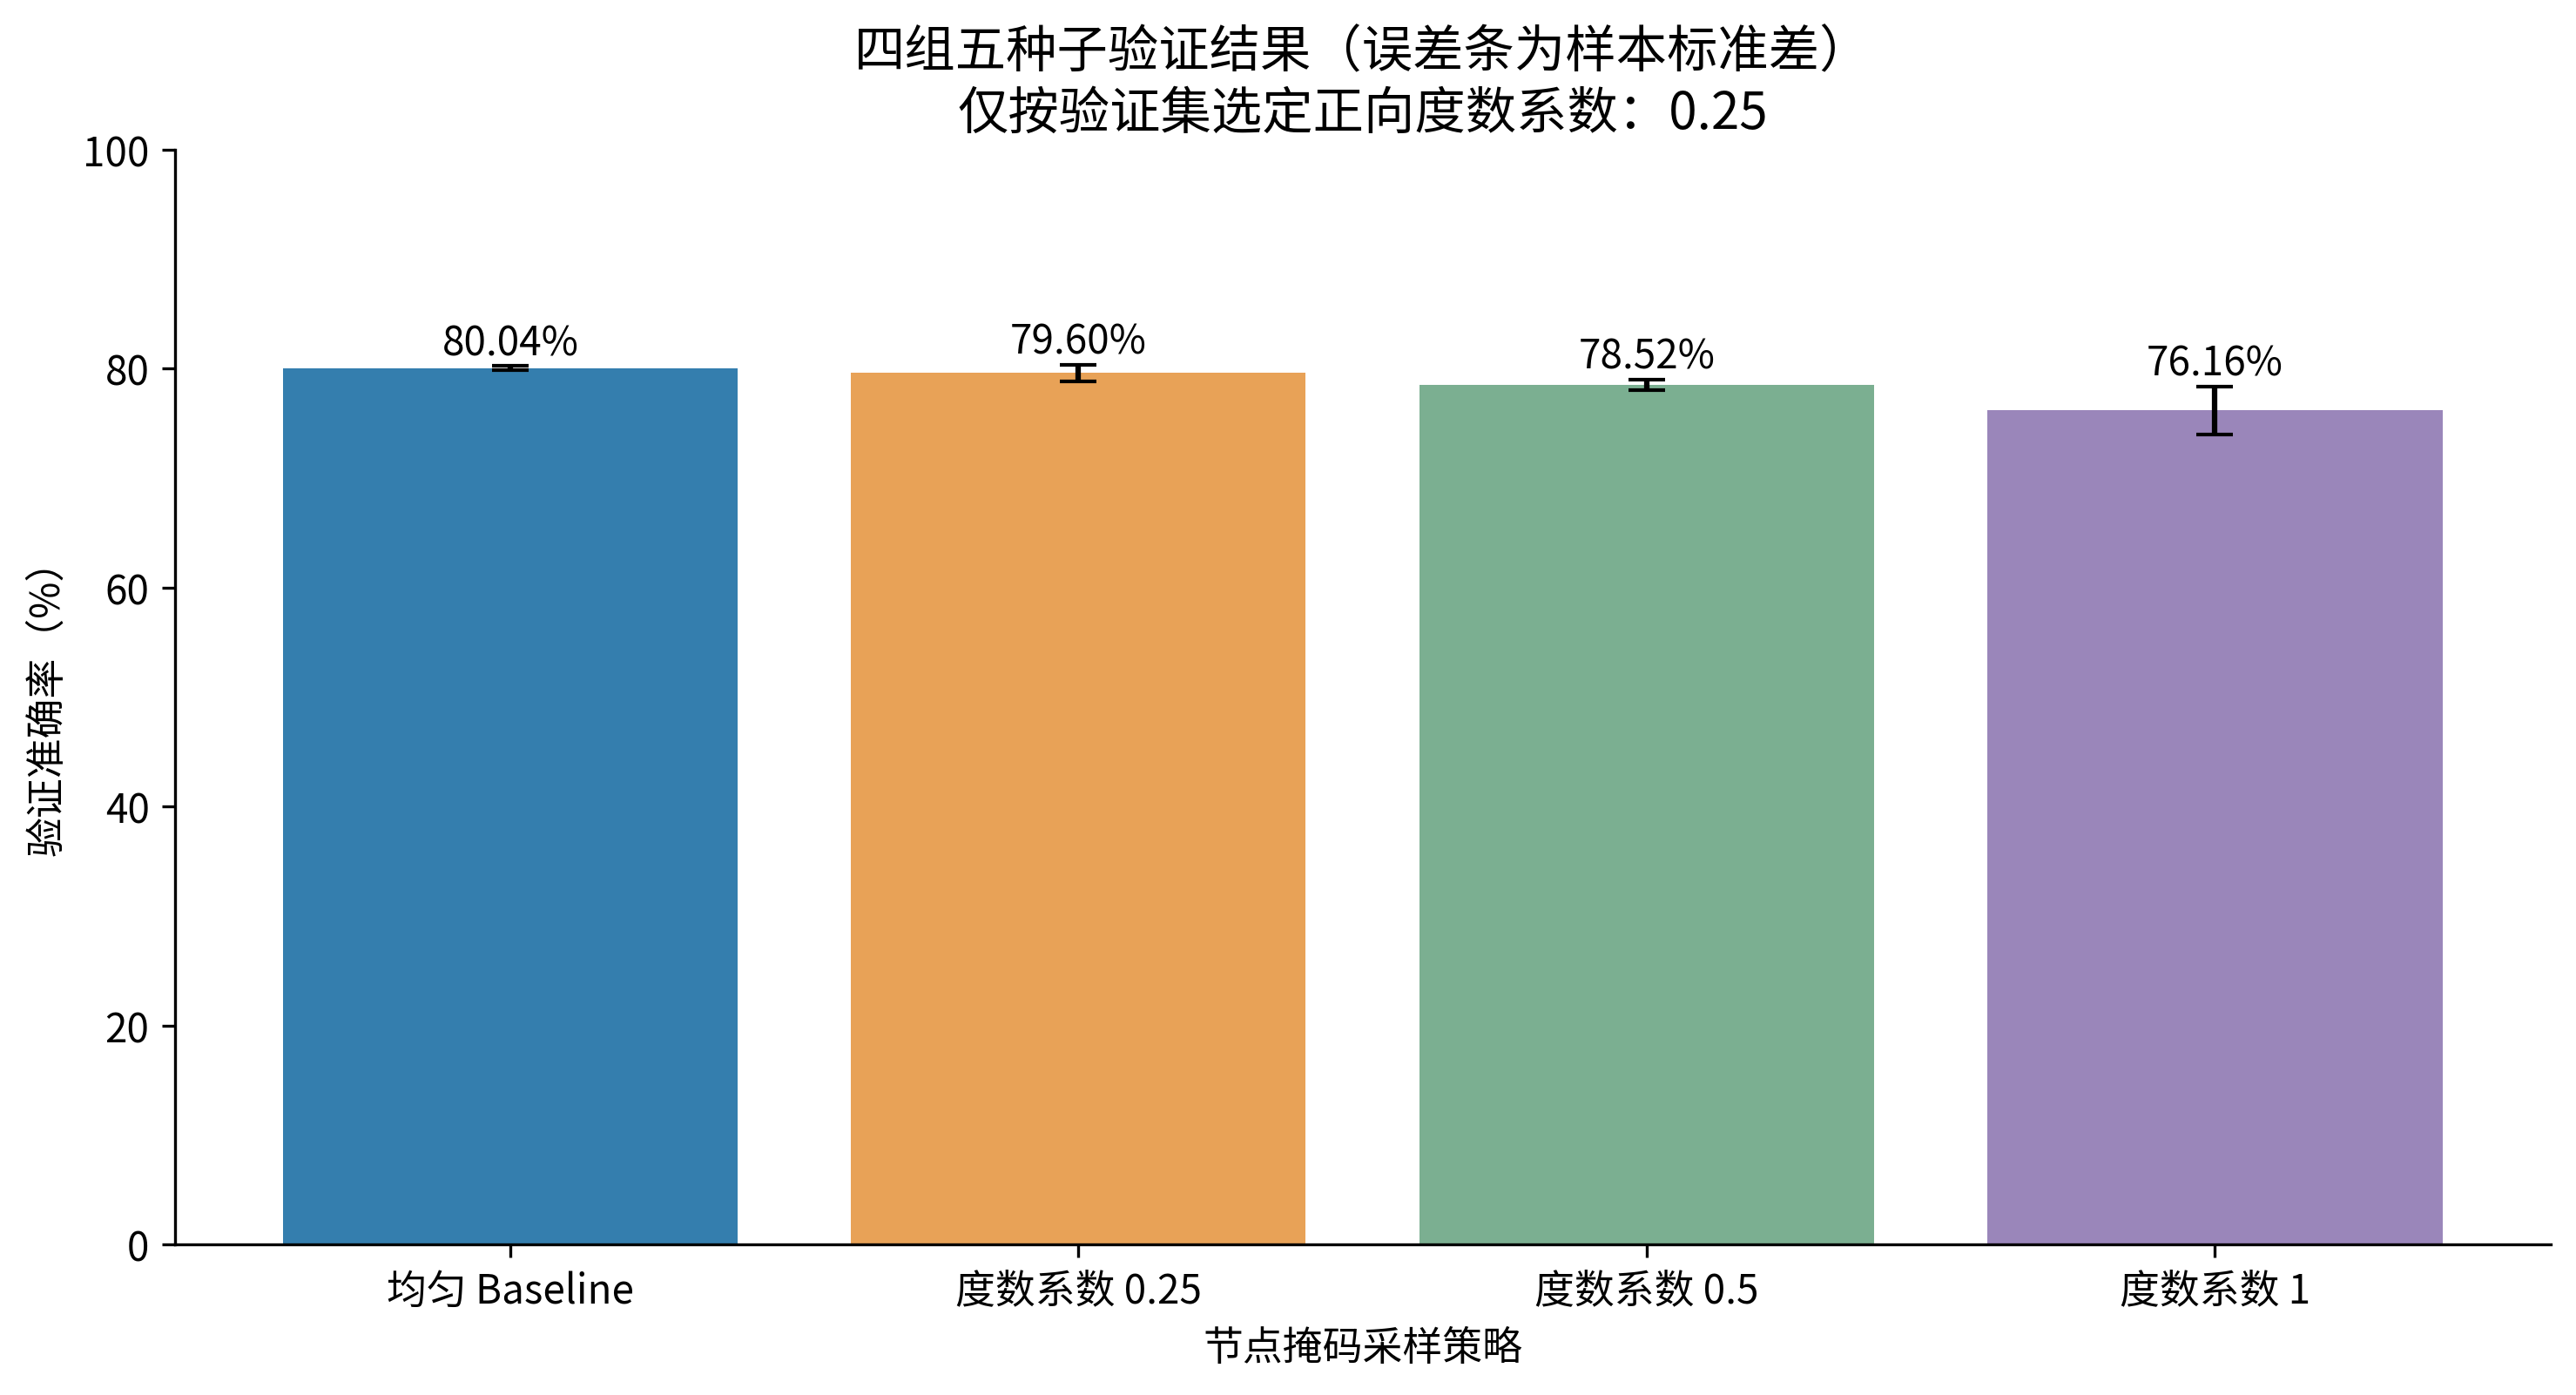
\includegraphics[width=0.88\linewidth]{../figures/M2/validation_comparison.png}
\caption{四组最终Probe最佳验证准确率的五种子均值及样本SD。0.25只在预设正向系数中最好，全部正向方案均低于控制组。}\label{fig:m2-validation}
\end{figure}

\subsection{最终测试与逐种子配对比较}
表\ref{tab:m2-paired}和图\ref{fig:m2-paired}保留五个种子的一一配对结果。定义每对变化为
\begin{equation}\label{eq:paired}
\Delta_s=100\left(a_{0.25,s}-a_{0,s}\right)\quad\text{（百分点）},
\end{equation}
其中$a$取0--1比例。控制组测试均值为84.20\%，样本SD为0.367423个百分点；0.25为82.92\%，样本SD为1.666433个百分点。平均配对变化为$-1.28$个百分点，配对差值的样本SD为1.682855个百分点。后者由五个差值计算，不是简单将两组SD相减。
\begin{table}[tbp]
\centering\small
\caption{M2最终测试的五种子配对。Accuracy单位为\%，差值单位为百分点。}\label{tab:m2-paired}
\begin{tabular}{rrrr}\toprule
Seed & 均匀控制组 & Degree-aware 0.25 & $\Delta_s$\\\midrule
0 & 84.20 & 80.10 & $-4.10$\\
1 & 84.80 & 83.50 & $-1.30$\\
2 & 84.10 & 84.00 & $-0.10$\\
3 & 84.10 & 84.20 & $+0.10$\\
4 & 83.80 & 82.80 & $-1.00$\\\midrule
均值 & 84.20 & 82.92 & $-1.28$\\
样本SD & 0.37 & 1.67 & 1.68\\\bottomrule
\end{tabular}
\end{table}
\begin{figure}[tbp]
\centering
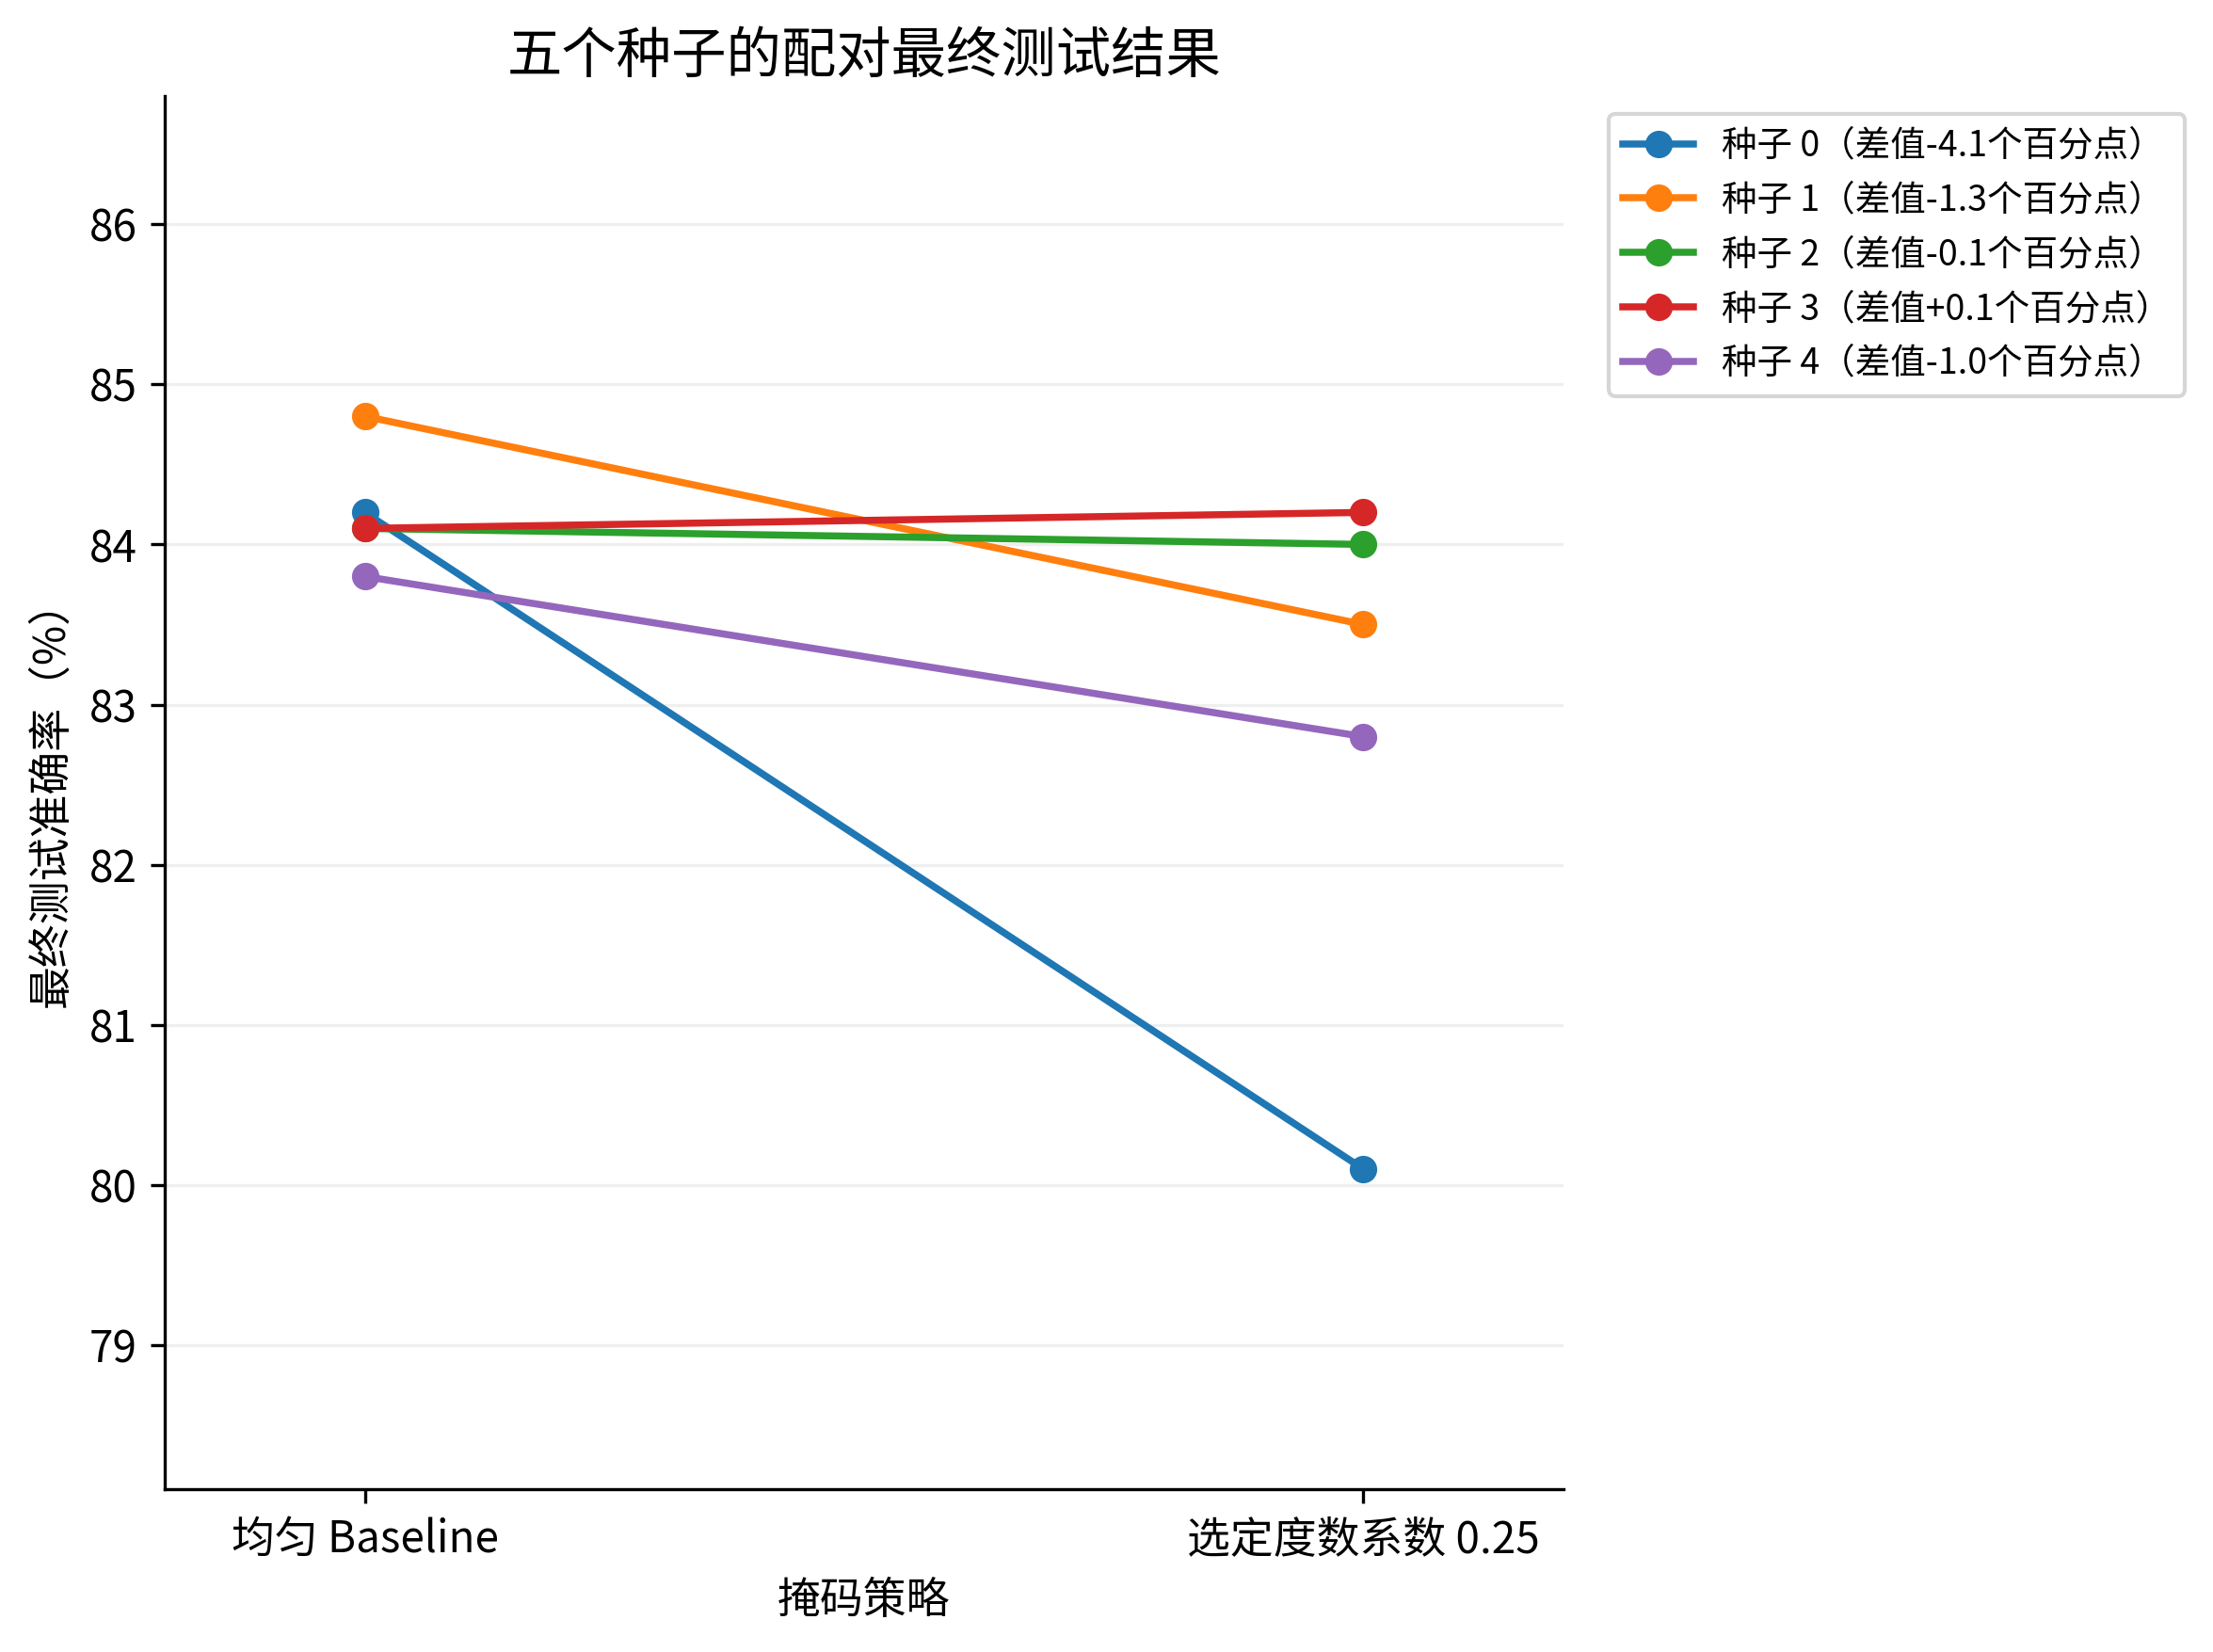
\includegraphics[width=0.88\linewidth]{../figures/M2/paired_test_accuracy.png}
\caption{控制组与0.25方案的逐种子配对测试结果。每条线对应同一seed，纵轴采用局部范围以展示差异，全部五对均保留。}\label{fig:m2-paired}
\end{figure}

五对中四对下降，一对提高0.10个百分点；seed0下降4.10个百分点，是本次波动的重要组成部分。不能仅展示seed3的小幅提高，也不能因seed0不利而重训或删除。该结果未支持本次配置下的平均性能改善假设，但仅五对重复不足以据此作普遍性结论或充分的统计推断。

\subsection{度数感知掩码是否真正生效}
全图度数最小为1、最大为168、均值3.898080、中位数3。分组边界在训练前仅按结构确定：在不拆分同度数节点的条件下，选择使三组人数相对$N/3$平方偏差之和最小的两个边界，得到低度数1--2、中度数3--4、高度数5--168，人数分别为1068、942、698。因此这些组不是严格等人数的三分位。

设$V_g$为度数组$g$的节点集合，$c_i$为节点$i$在1500轮中被选中的次数。组内实际掩码率为
\begin{equation}\label{eq:mask-rate}
c_i=\sum_{t=1}^{1500}\mathbf1\{i\in M_t\},\quad
\widehat r_g=\frac{\sum_{i\in V_g}c_i}{1500|V_g|},\quad
\overline c_g=\frac{\sum_{i\in V_g}c_i}{|V_g|}.
\end{equation}
它回答“该组一个节点在一轮中平均多常被掩码”，不同于该组占全部掩码选择的份额，后者分母为$1500\times1354$。

图\ref{fig:m2-mask}显示均匀控制组各组掩码率均接近50\%；0.25时低、中、高度数组分别约为45.68\%、50.52\%、55.90\%。对应平均被选次数为685.27、757.84、838.47，而控制组约为750.01、749.65、750.46。系数进一步增大至0.5和1.0时，高度数组掩码率达到61.67\%和71.98\%，低度数组降为41.56\%和34.14\%。每轮总选点始终为1354，故这种偏移不是由额外增加训练目标数量造成。实际频率说明度数权重确实改变了采样分布，实现生效与分类收益应分别判断。
\begin{figure}[tbp]
\centering
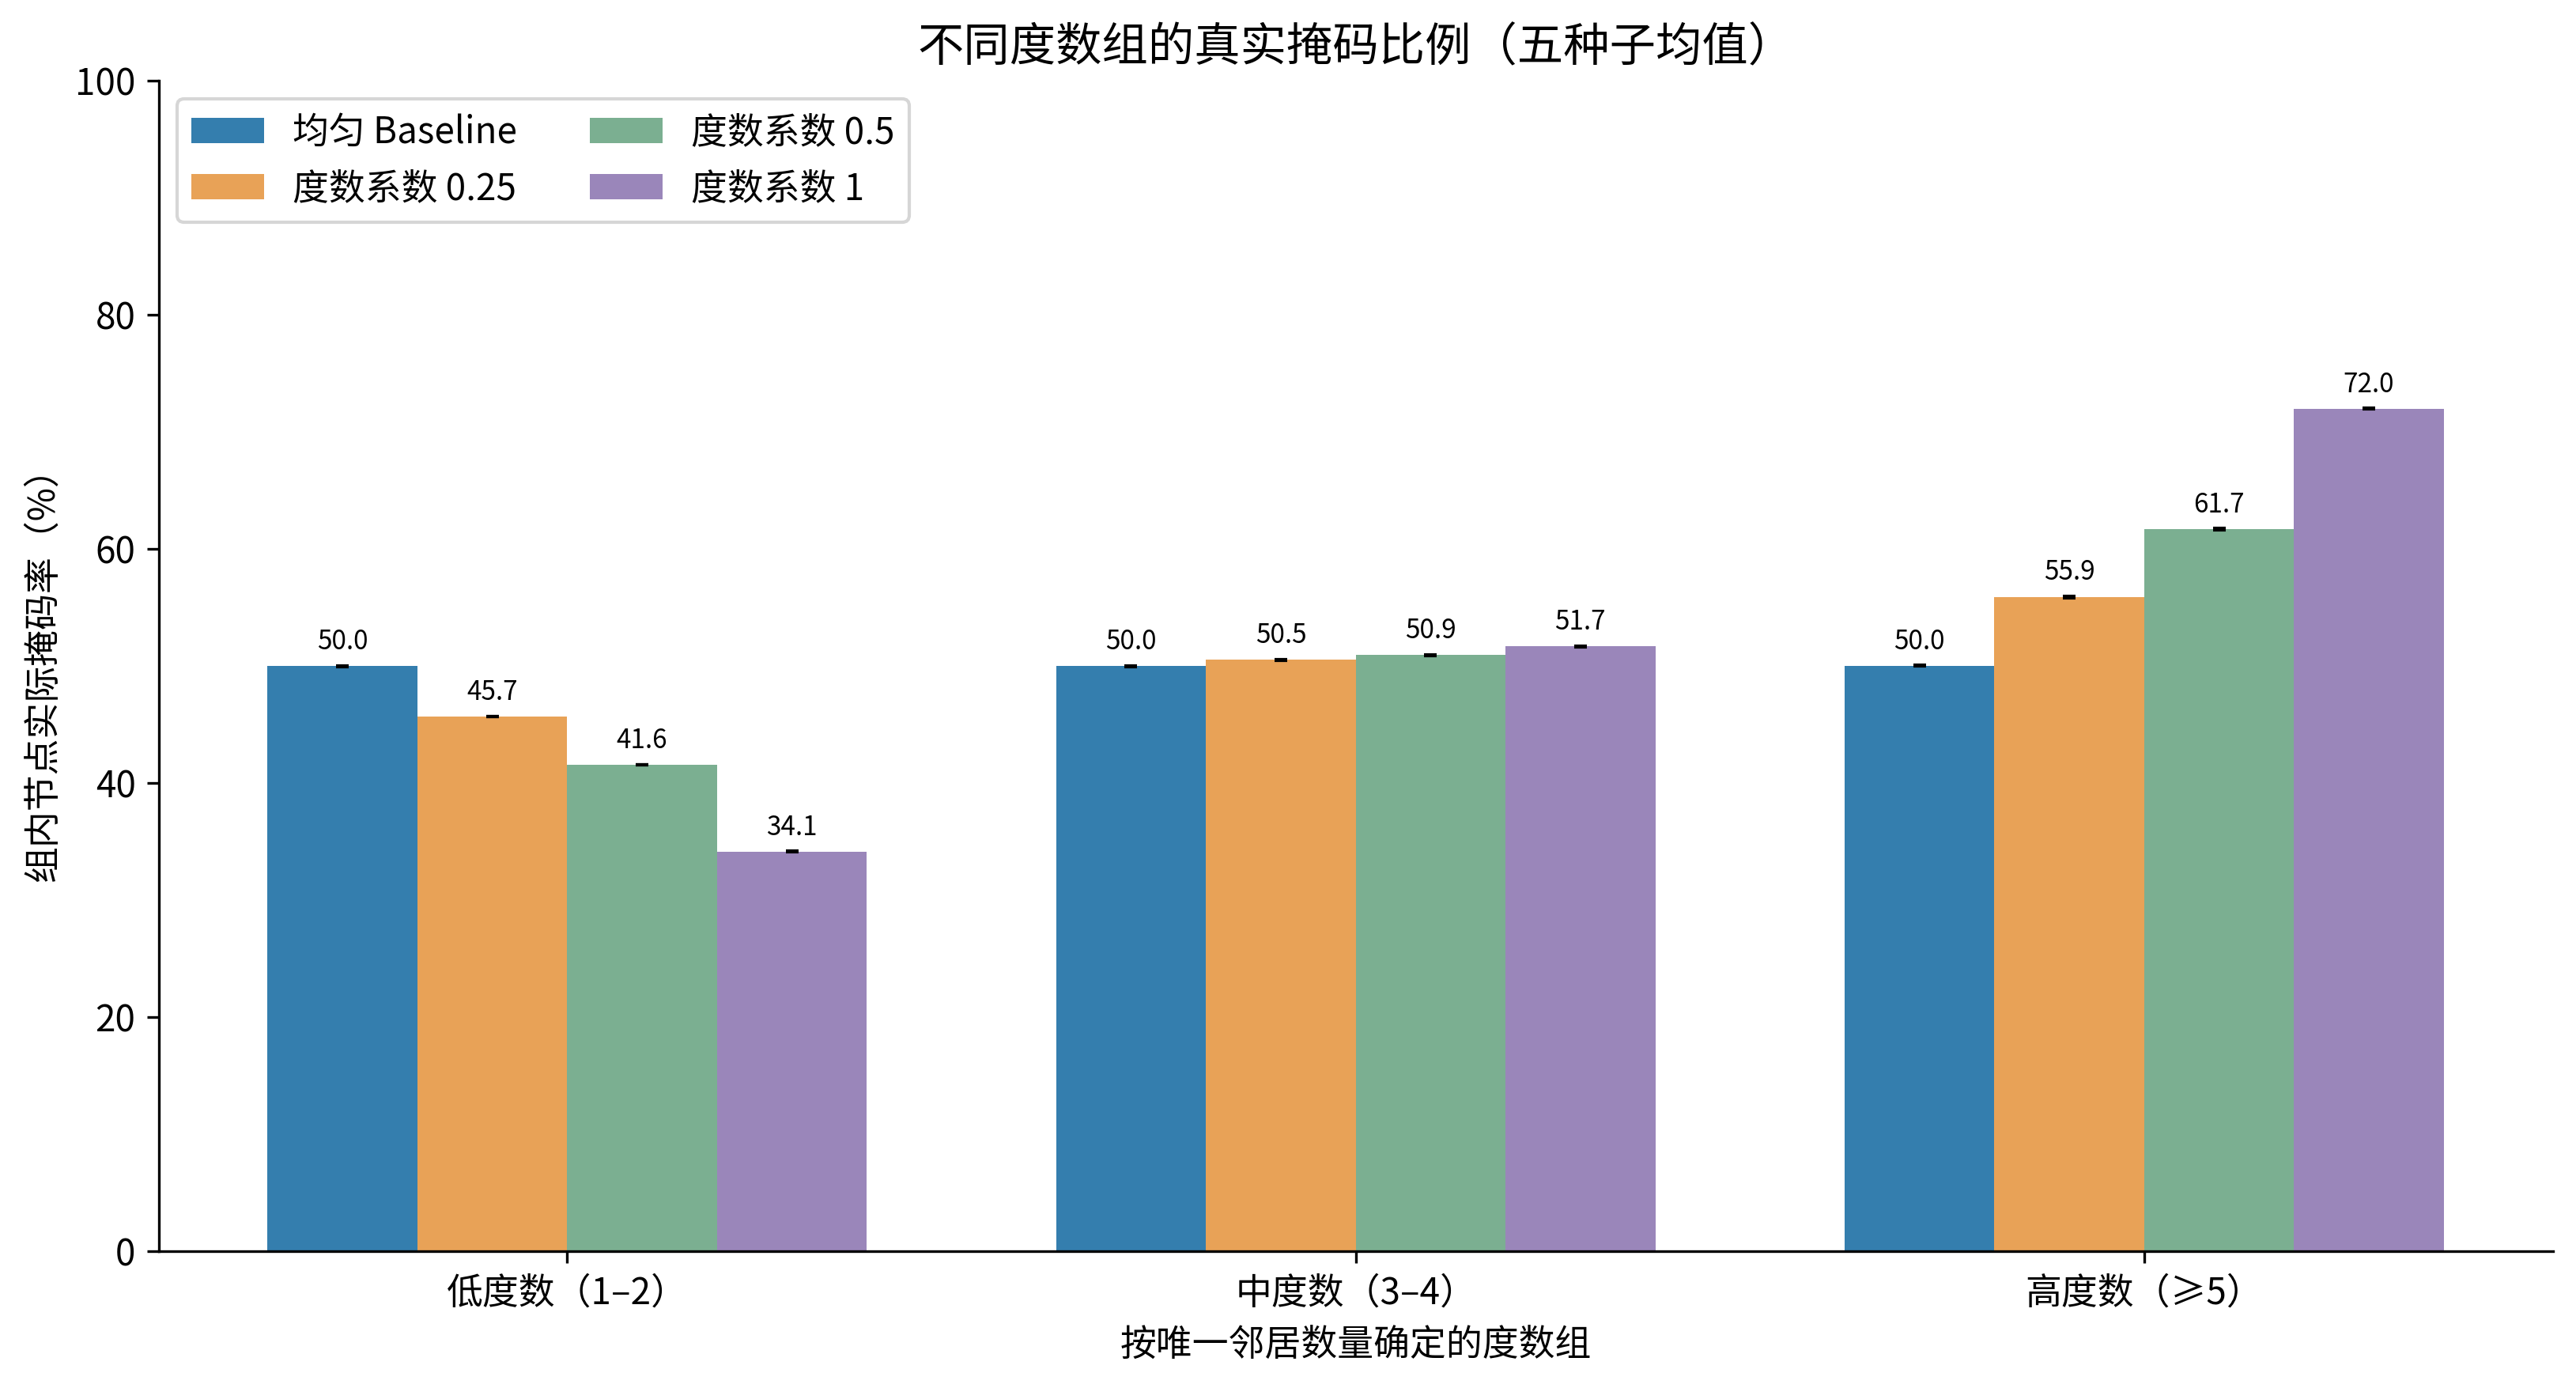
\includegraphics[width=0.92\linewidth]{../figures/M2/degree_mask_rates.png}
\caption{各度数组的组内实际掩码率，使用每次1500轮的逐节点计数汇总。柱为五种子均值，误差条为样本SD；所有组均固定每轮1354个节点。}\label{fig:m2-mask}
\end{figure}

\subsection{不同度数组的分类表现}
最终参数封存后，使用同一次测试保存的预测计算分组准确率，没有再次运行模型或依分组测试结果重选系数。对于组$g$，
\begin{equation}\label{eq:group-accuracy}
\operatorname{Acc}_g=\frac{\sum_{i\in V_g\cap V_{\rm te}}\mathbf1\{\widehat y_i=y_i\}}
{|V_g\cap V_{\rm te}|}.
\end{equation}
表\ref{tab:degree-groups}和图\ref{fig:m2-groups}显示三组平均均下降，低、中、高组分别下降0.95、约1.38、约1.67个百分点。高度数组虽增加了掩码监督，却没有取得预期的平均分类收益。中度数组Accuracy高于低度数组是当前节点集合上的观察，不能解释为度数增大必然提升分类。
\begin{table}[tbp]
\centering\small
\caption{度数组规模与最终测试结果。正确数为同一测试划分的五次预测合计；Accuracy为五种子均值，不把重复评价次数当独立节点数。}\label{tab:degree-groups}
\footnotesize
\setlength{\tabcolsep}{4pt}
\begin{tabular}{lrrrrr}\toprule
度数组 & 全图人数 & 测试人数/seed & 控制正确数 & 0.25正确数 & Accuracy：控制/0.25\\\midrule
低：1--2 & 1068 & 400 & 1575/2000 & 1556/2000 & 78.75/77.80\%\\
中：3--4 & 942 & 348 & 1543/1740 & 1519/1740 & 88.68/87.30\%\\
高：5--168 & 698 & 252 & 1092/1260 & 1071/1260 & 86.67/85.00\%\\\bottomrule
\end{tabular}
\end{table}
\begin{figure}[tbp]
\centering
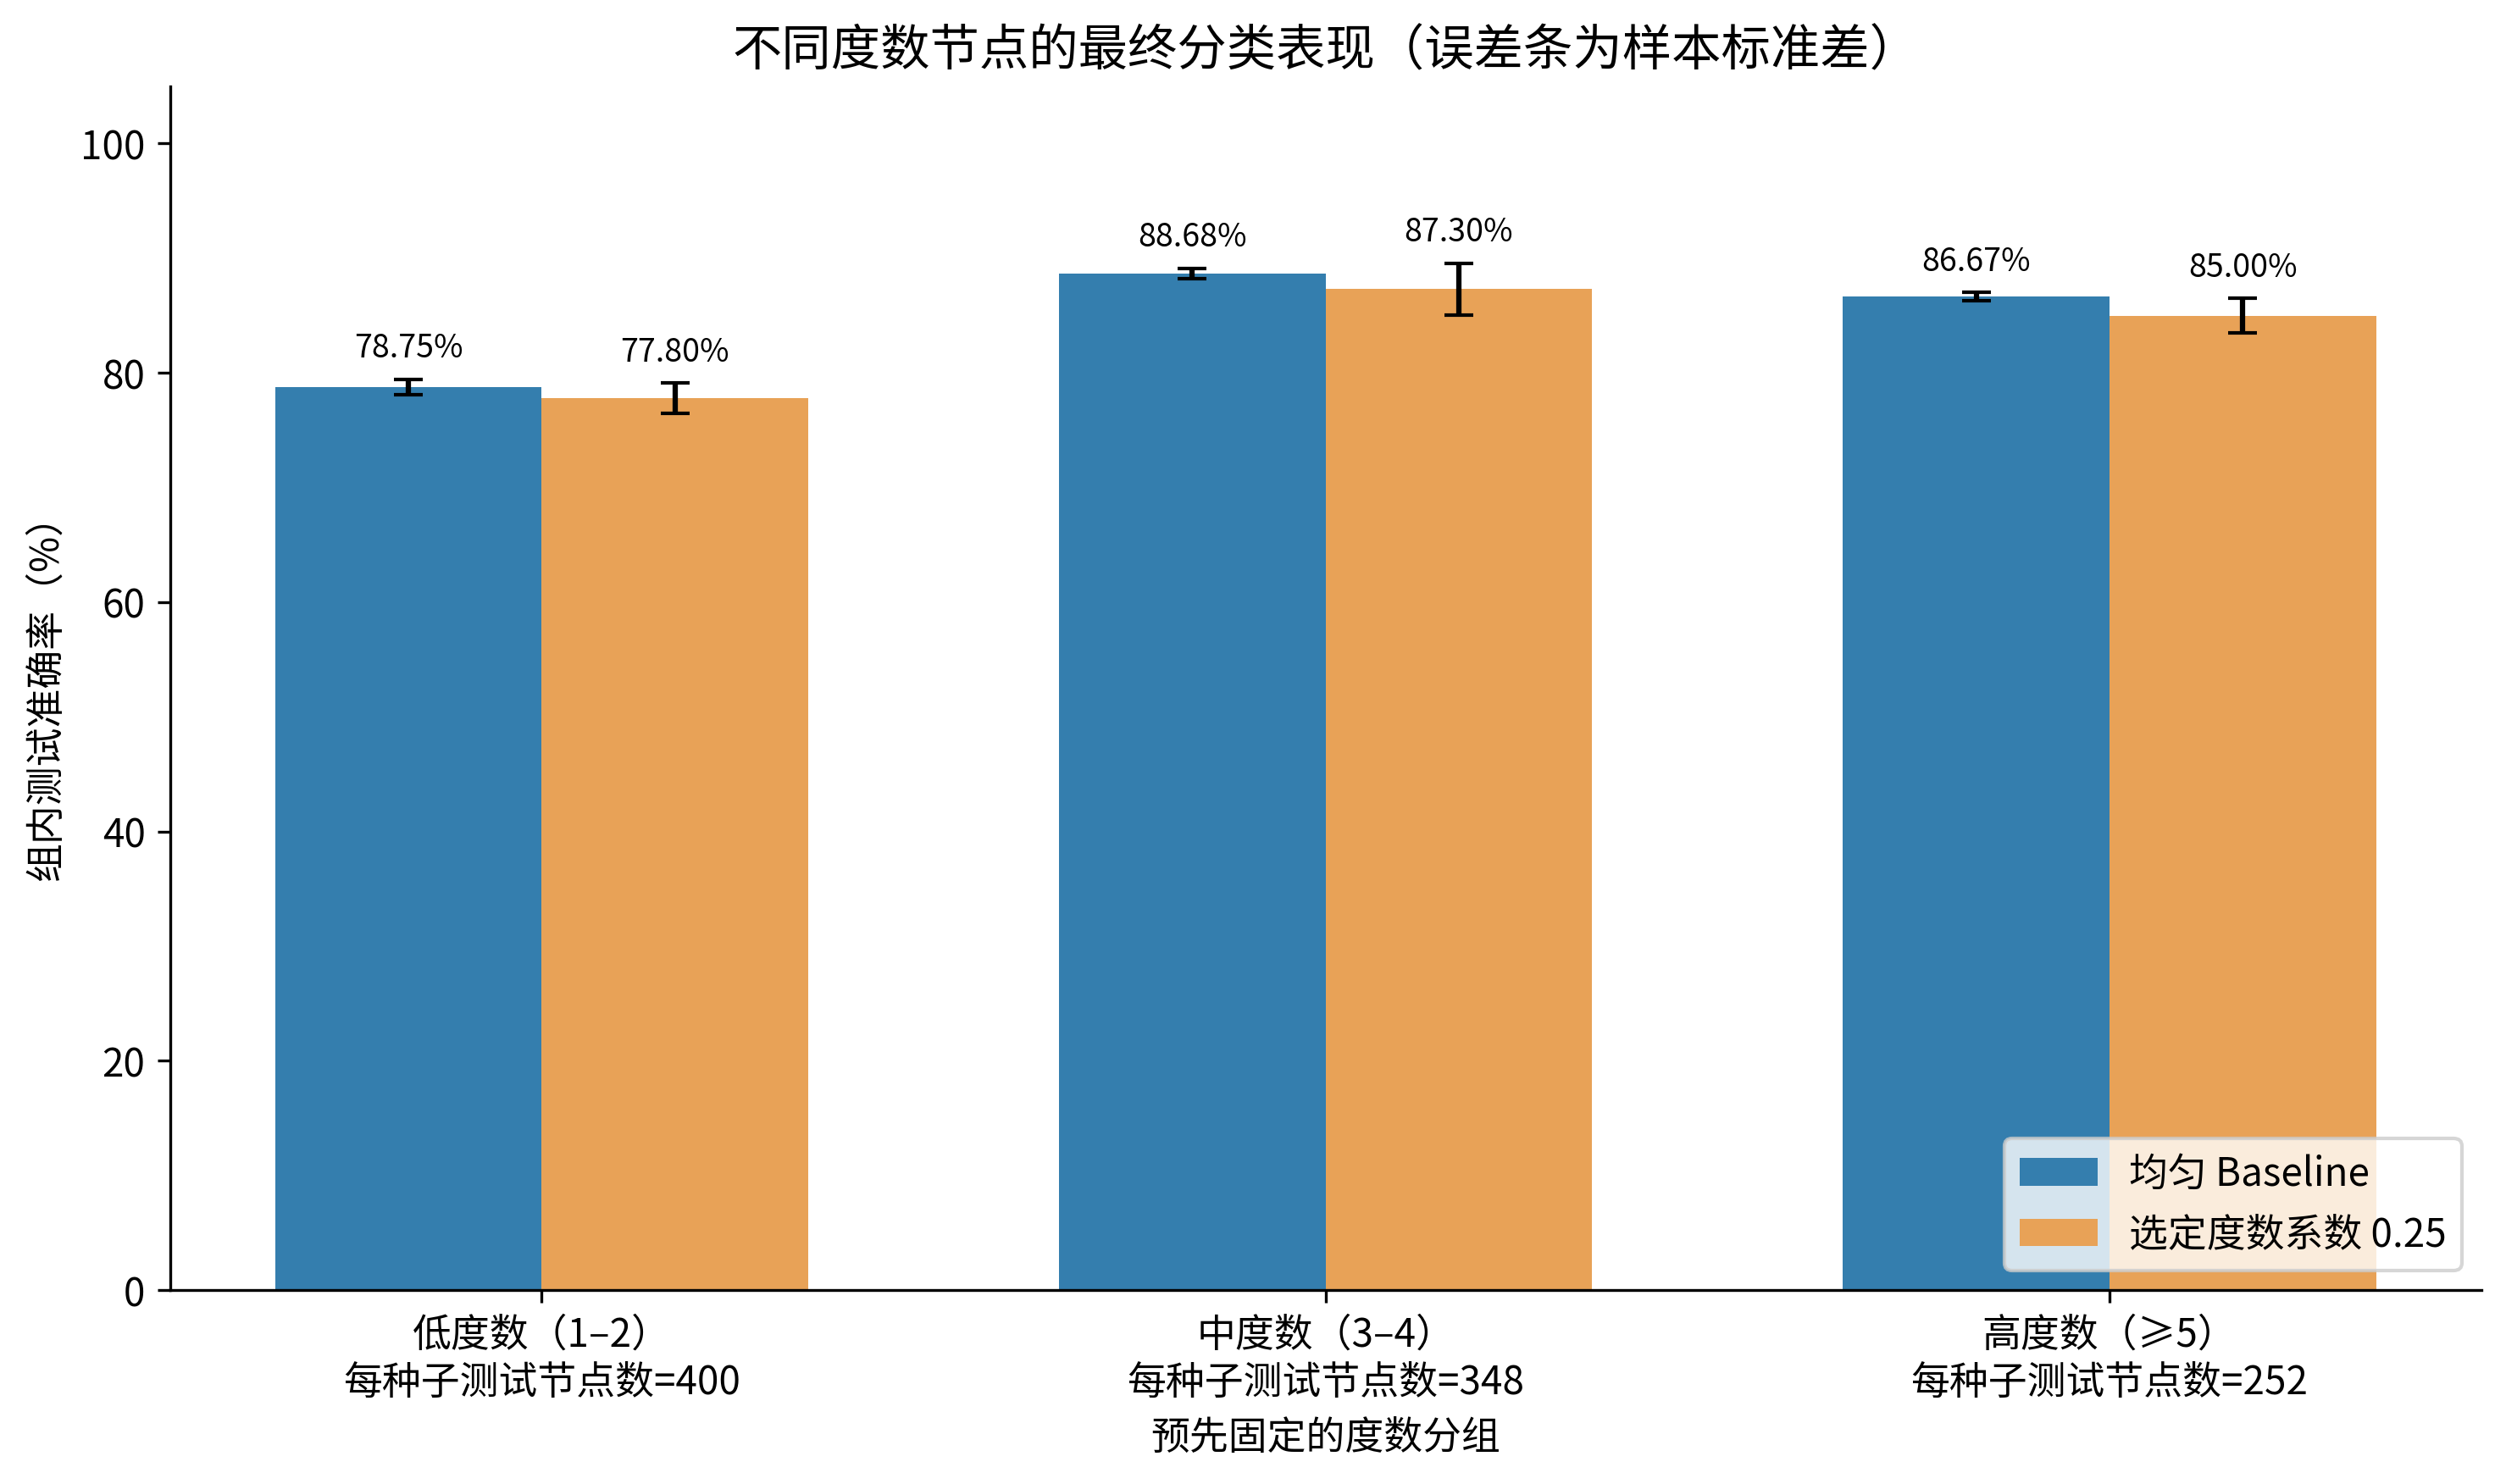
\includegraphics[width=0.90\linewidth]{../figures/M2/degree_classification.png}
\caption{控制组与0.25的度数组测试准确率。柱为五种子均值，误差条为样本SD；每seed固定使用400、348、252个测试节点。分组边界未使用测试标签。}\label{fig:m2-groups}
\end{figure}

五个种子共用同一public split，因此例如低度数组的2000次评价仍来自固定400个节点，不构成2000个独立测试样本。各组规模不均，组内差异仅用于描述哪些节点集合可能受影响，不足以证明单一作用机制。

\subsection{Loss与训练开销}
图\ref{fig:m2-loss}及表\ref{tab:m2-cost}显示，控制组最后100轮的平均SCE为0.402125，0.25方案为0.414893；0.5和1.0分别为0.425383和0.442083。本次没有“降低重建Loss但分类退化”的现象，重建数值也未改善。由于采样使参与损失的节点分布改变，不同方案的SCE并非同一组等难度目标上的泛化误差，不能用其绝对大小代替分类评价。
\begin{figure}[tbp]
\centering
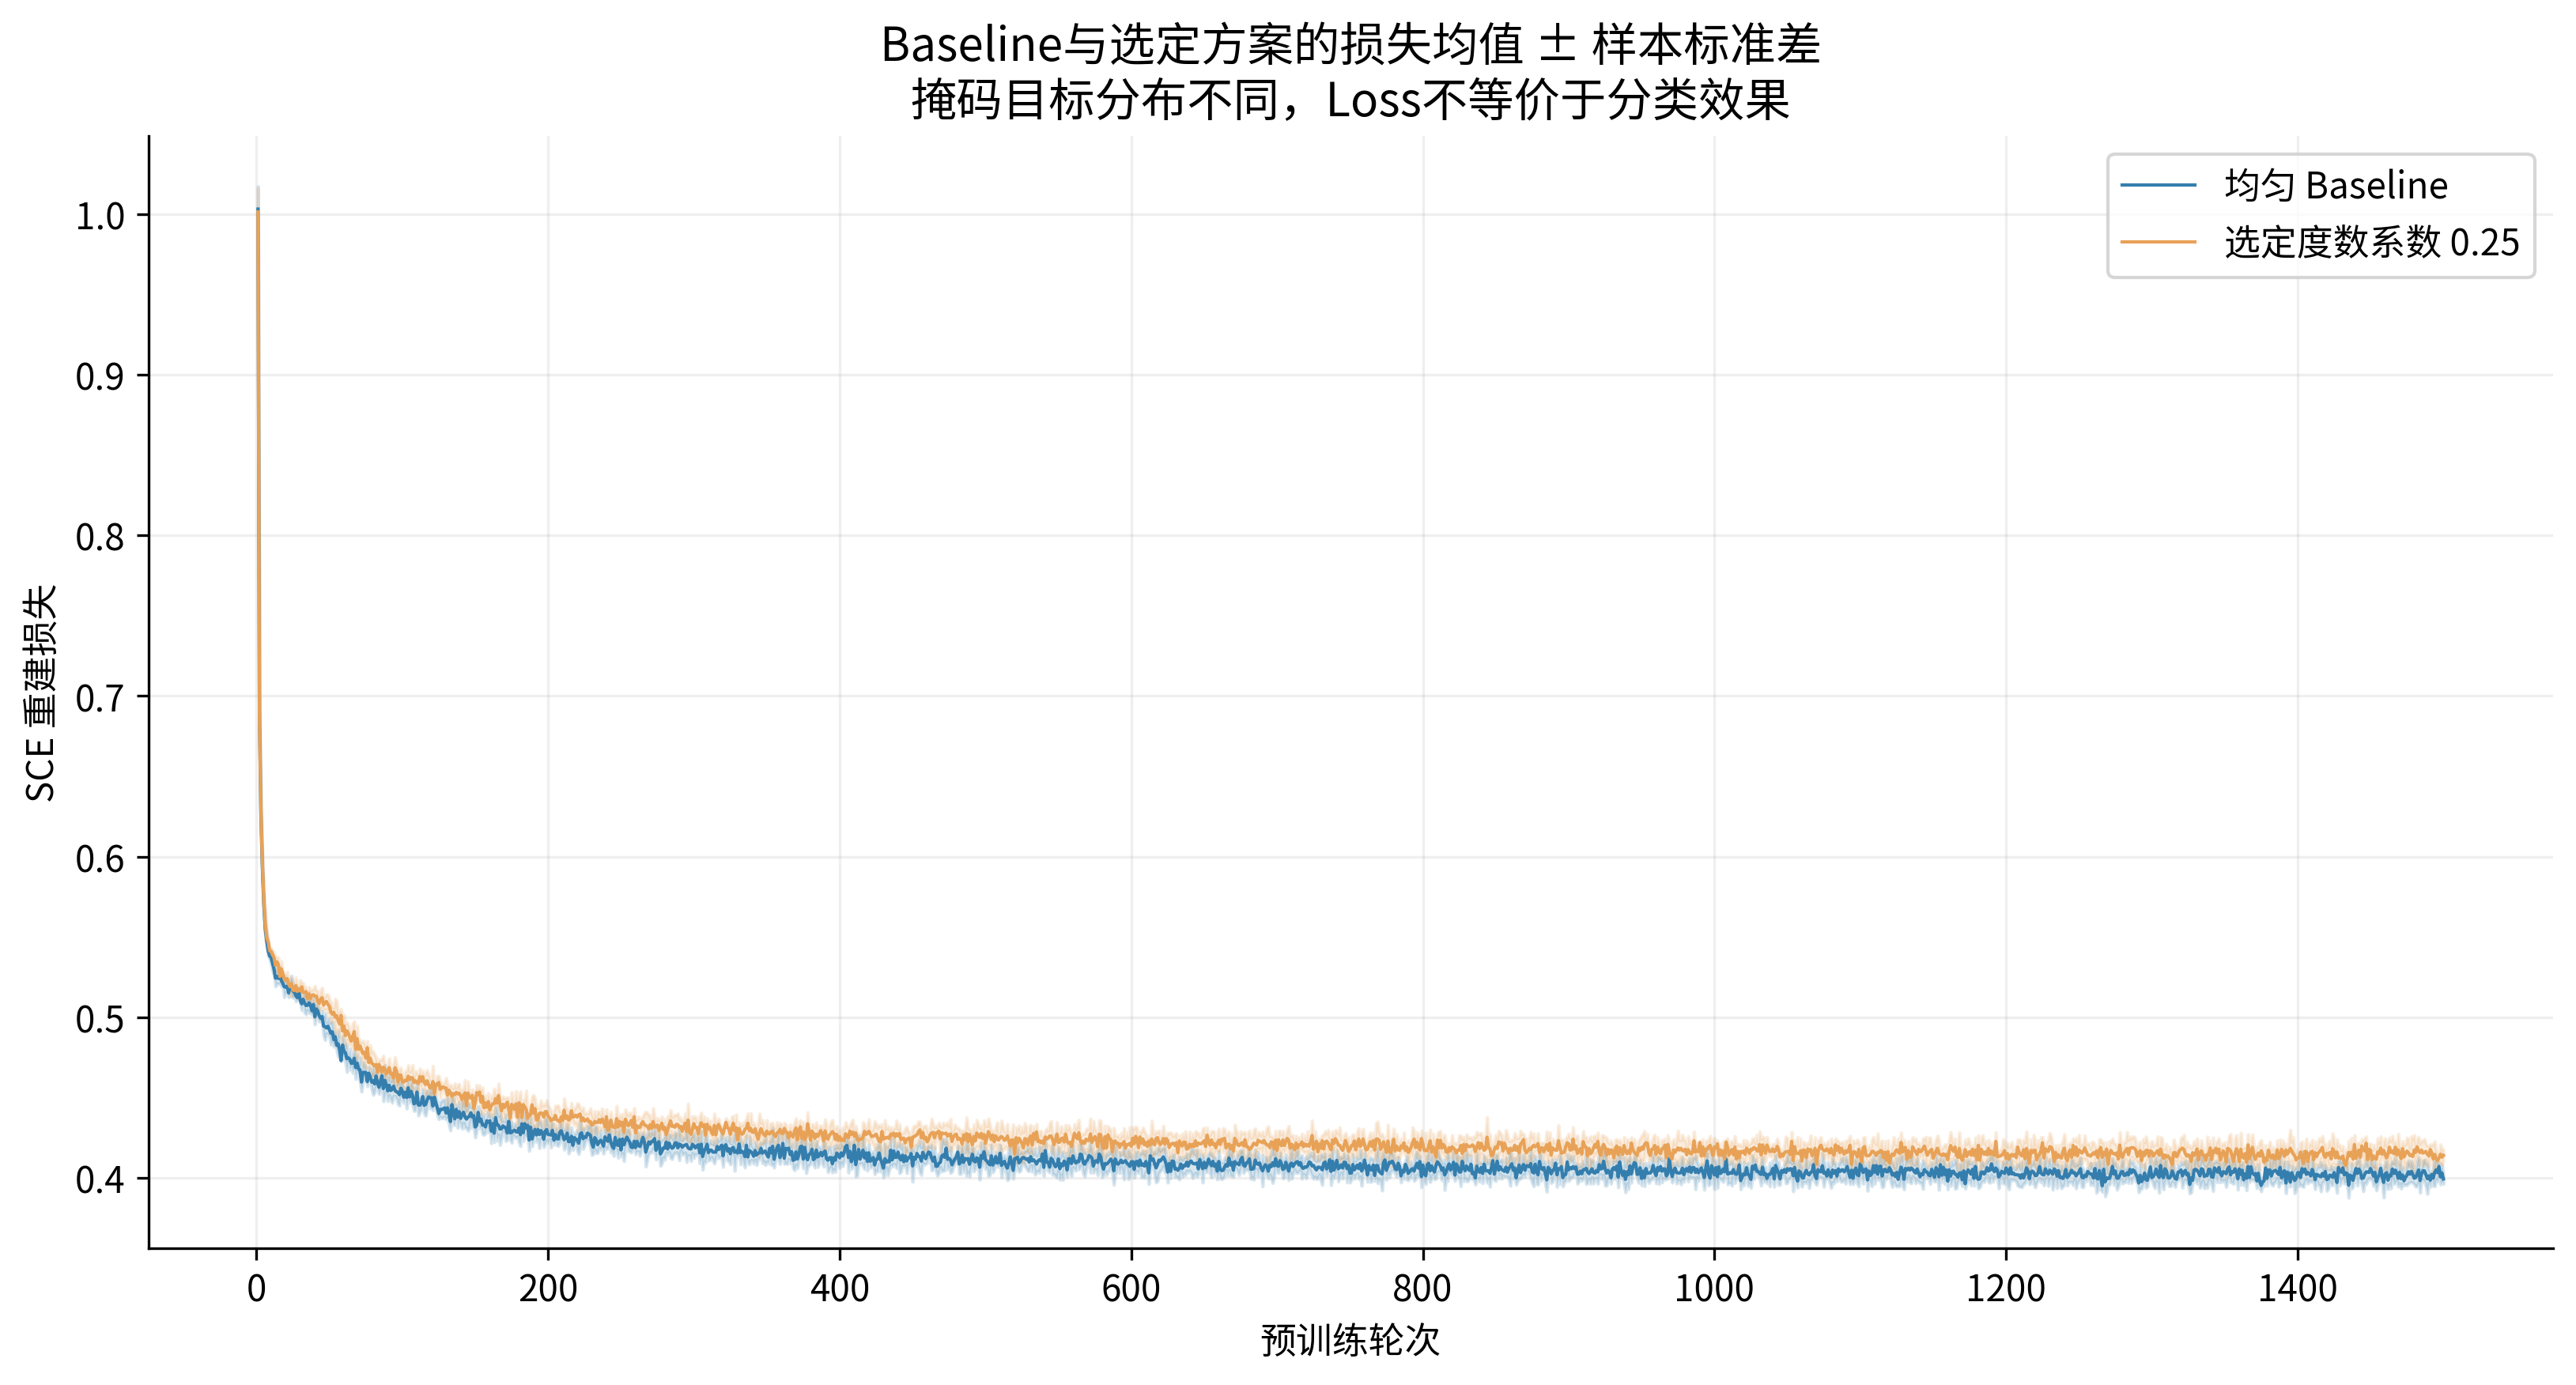
\includegraphics[width=0.90\linewidth]{../figures/M2/loss_curves.png}
\caption{M2控制组与0.25的预训练SCE。曲线为逐轮五种子均值，阴影为样本SD，两者使用不同掩码目标分布。}\label{fig:m2-loss}
\end{figure}
\begin{table}[tbp]
\centering\small
\caption{M2训练过程统计。末100轮Loss先对各seed取均值再跨seed平均；时间为worker均值，峰值为PyTorch allocated张量显存的跨seed平均。}\label{tab:m2-cost}
\begin{tabular}{rrrr}\toprule
$\alpha_d$ & 末100轮SCE & 时间/s & 峰值显存/MiB\\\midrule
0 & 0.402125 & 26.993 & 472.73\\
0.25 & 0.414893 & 28.219 & 472.73\\
0.5 & 0.425383 & 27.538 & 472.69\\
1.0 & 0.442083 & 29.380 & 472.73\\\bottomrule
\end{tabular}
\end{table}

M2时间包含数据、初始化、预训练、全部Probe和保存，不包含模块导入、启动前GPU资源检查与后续最终测试。0.25比控制组均值增加约1.23秒，但服务器负载、CPU采样和日志校验均会影响计时，且并非专门的性能基准，不能据此精确归因采样开销。峰值张量显存约473MiB，未包含所有CUDA上下文或其他用户进程。M1计时包含导入，与M2边界不同，不作跨批次加速比较。
